\documentclass{rapportECL}
\usepackage{lipsum}
\usepackage{overpic}
\usepackage{xcolor}
\usepackage{graphicx}
\usepackage{tcolorbox}
\usepackage{enumitem}
\usepackage{amsmath}
\usepackage{multirow}
\usepackage{booktabs}
\usepackage{tabularx}
\usepackage{siunitx}
\usepackage{hyperref}
\usepackage{caption}
\usepackage{subcaption}


\sisetup{per-mode=symbol, exponent-product=\cdot, separate-uncertainty=true}

\begin{document}

%----------- Informations du rapport ---------
\titre{Homogénéisation analytique et numérique d'un composite TRC.} 
\UE{Méthodes Numériques Avancées}
\enseignant{Anicet DANSOU}
\eleves{[TONGUE Kevin] \\ [KAMDEM TCHOMTHOUA Gaston]}


%----------- Initialisation -------------------
\fairemarges
\fairepagedegarde
\newpage
\tabledematieres

\section*{Introduction}

\subsection*{Contexte et problématique}

Les matériaux composites à renfort textile (TRC - Textile Reinforced Concrete) représentent une alternative prometteuse aux composites polymères (FRP) traditionnels dans le domaine de la réhabilitation structurale. Leurs avantages incluent une meilleure compatibilité avec les substrats minéraux, une résistance au feu améliorée et un impact environnemental réduit \cite{Yosef2021,Valeri2020}.

L'objectif de ce projet est la caractérisation multi-échelle des propriétés mécaniques effectives d'une plaque TRC unidirectionnelle, en combinant des approches analytiques et numériques. Le matériau étudié est constitué d'une matrice minérale renforcée par des fibres de carbone T700SC alignées.

\subsection*{Données du problème}

\begin{table}[h]
\centering
\caption{Propriétés géométriques et matériaux de la plaque TRC}
\begin{tabular}{lccc}
\toprule
Paramètre & Symbole & Valeur & Unité \\
\midrule
Longueur de la plaque & $L$ & 550 & \si{\milli\meter} \\
Largeur de la plaque & $l$ & 99 & \si{\milli\meter} \\
Épaisseur & $e$ & 6,69 & \si{\milli\meter} \\
Nombre de mèches & $N$ & 188,3 & \si{\per\meter} \\
Section d'une fibre & $A_f$ & 8,31×10^{-12} & \si{\meter^2} \\
\bottomrule
\end{tabular}
\end{table}

\textbf{Fibres de carbone T700SC 12K}:
\begin{itemize}
\item Module d'Young: $E_f = 200$ \si{\giga\pascal} (valeur corrigée)
\item Résistance en traction: 3300 \si{\mega\pascal}
\item Allongement à rupture: 2\%
\end{itemize}

\textbf{Matrice minérale}:
\begin{itemize}
\item Module d'Young: $E_m = 25$ \si{\giga\pascal}
\item Résistance en traction: 4,5-5 \si{\mega\pascal}
\item Allongement à rupture: 0,02-0,03\%
\end{itemize}

\section{Volume Élémentaire Représentatif (VER)}

\subsection{Définition du VER}

Pour une plaque TRC unidirectionnelle, le VER est défini comme le plus petit volume permettant de représenter statistiquement la microstructure du composite. Compte tenu de la périodicité de la distribution des fibres, un parallélépipède contenant une seule fibre est choisi (Figure \ref{fig:ver}).

\begin{figure}[h]
\centering
\includegraphics[width=0.5\textwidth]{VER_schema.png}
\caption{Volume Élémentaire Représentatif pour la plaque TRC}
\label{fig:ver}
\end{figure}

\subsection{Caractéristiques géométriques}

\begin{itemize}
\item Dimensions: $L_x \times L_y \times e$ avec $e = 6,69$ \si{\milli\meter}
\item Distance inter-fibres: $d = 1/N = 5,31$ \si{\milli\meter}
\item Fraction volumique de fibres: 
\[
v_f = \frac{N \times A_f}{e} = \frac{188,3 \times 8,31\times10^{-12}}{0,00669} \approx 2,34\%
\]
\item Fraction volumique de matrice: $v_m = 1 - v_f \approx 97,66\%$
\end{itemize}

\section{Homogénéisation analytique}

\subsection{Méthodes de Voigt et Reuss}

\subsubsection{Module longitudinal $E_1$}

\textbf{Voigt (déformation uniforme)}:
\[
E_1^{\text{Voigt}} = v_f E_f + v_m E_m = 0,0234 \times 200 + 0,9766 \times 25 = 29,21\ \si{\giga\pascal}
\]

\textbf{Reuss (contrainte uniforme)}:
\[
\frac{1}{E_1^{\text{Reuss}}} = \frac{v_f}{E_f} + \frac{v_m}{E_m} = \frac{0,0234}{200} + \frac{0,9766}{25} = 0,0391
\]
\[
E_1^{\text{Reuss}} = 25,57\ \si{\giga\pascal}
\]

\subsubsection{Module transverse $E_2$}

Pour le module transverse, l'approche de Reuss est plus appropriée:
\[
\frac{1}{E_2} = \frac{v_f}{E_f} + \frac{v_m}{E_m} \Rightarrow E_2 \approx 25,57\ \si{\giga\pascal}
\]

\subsubsection{Coefficient de Poisson $\nu_{12}$}

\[
\nu_{12} = v_f \nu_f + v_m \nu_m
\]
En prenant $\nu_f = 0,2$ (carbone) et $\nu_m = 0,18$ (matrice):
\[
\nu_{12} = 0,0234 \times 0,2 + 0,9766 \times 0,18 = 0,1805
\]

\subsection{Discussion des résultats analytiques}

\begin{table}[h]
\centering
\caption{Propriétés effectives par différentes méthodes}
\begin{tabular}{lccc}
\toprule
Propriété & Voigt & Reuss & Écart relatif \\
\midrule
$E_1$ (GPa) & 29,21 & 25,57 & 14,2\% \\
$E_2$ (GPa) & 29,21* & 25,57 & 14,2\% \\
\bottomrule
\end{tabular}
\end{table}

\begin{itemize}
\item La méthode de Voigt surestime les propriétés effectives (borne supérieure)
\item La méthode de Reuss sous-estime les propriétés (borne inférieure)
\item Pour les composites unidirectionnels, la loi des mélanges (Voigt) donne une bonne approximation de $E_1$
\item L'anisotropie est modérée: $E_1/E_2 \approx 1,14$ (voisin de 1 car $v_f$ faible)
\end{itemize}

\subsection{Autres méthodes analytiques}

D'autres approches pourraient être utilisées pour affiner les prédictions:

\begin{enumerate}
\item \textbf{Méthode de Hashin-Shtrikman}: Fournit des bornes plus serrées que Voigt/Reuss pour les composites isotropes transverses.

\item \textbf{Méthode de Mori-Tanaka}: Prend en compte les interactions fibre-fibre via un formalisme d'inclusion. Particulièrement adaptée pour $v_f < 30\%$.

\item \textbf{Modèle cylindrique concentrique}: Modèle exact pour une fibre au centre d'un cylindre de matrice, applicable par éléments finis.
\end{enumerate}

\section{Homogénéisation numérique}

\subsection{Pertinence pour le TRC}

L'homogénéisation numérique présente plusieurs avantages pour les composites TRC:

\begin{itemize}
\item Prise en compte de la microstructure réelle (distribution, orientation)
\item Simulation des mécanismes d'endommagement à l'interface
\item Analyse des concentrations de contraintes locales
\item Validation des modèles analytiques simplifiés
\end{itemize}

\subsection{Modélisation du VER avec Abaqus}

\subsubsection{Protocole de simulation}
\paragraph{cas1:Détermination de E3}

\begin{enumerate}
\item \textbf{Géométrie}: VER 3D avec une fibre cylindrique centrée
\item \textbf{Maillage}: 
  \begin{itemize}
  \item Fibre: éléments hexaédriques linéaires (C3D8R)
  \item Matrice: éléments tétraédriques (C3D4)
  \item Taille caractéristique: 0,1 mm
  \end{itemize}
\item \textbf{Matériaux}: Élastique linéaire
  \begin{itemize}
  \item Fibre: $E_f = 200$ GPa, $\nu_f = 0,2$
  \item Matrice: $E_m = 25$ GPa, $\nu_m = 0,18$
  \end{itemize}
\item \textbf{Conditions aux limites}: Périodiques sur les faces latérales
\item \textbf{Chargements}: Déplacements imposés pour extraire
  \begin{itemize}
  \item Encastrement suivant une face perpendiculaire à la direction des fibres
  \item déplacement imposé sur la face opposée
  \item symétrie sur les faces dans la direction de la largeur

  \end{itemize}
\end{enumerate}
Nous avons dans un premier temps fait abstraction de la \textbf{la symétrie} qui modélise. une fois la démarche de modélisation terminée, la contrainte dans la direction du 3 et la déformation dans la direction 3 sont recueillis pour déterminer la contrainte équivalente en calculant la moyenne volumique. Il est à noter que cette repartions de contrainte est différente pour la matrice et pour la fibre. La contrainte est plus grande dans la matrice que dans la fibre et pareillement pour la contrainte. On suppose que la déformation est constante dans le matériau et on évalue le module de Young en faisant la moyenne volumique des contraintes dans le VER. 
\begin{figure}[H]
    \centering
    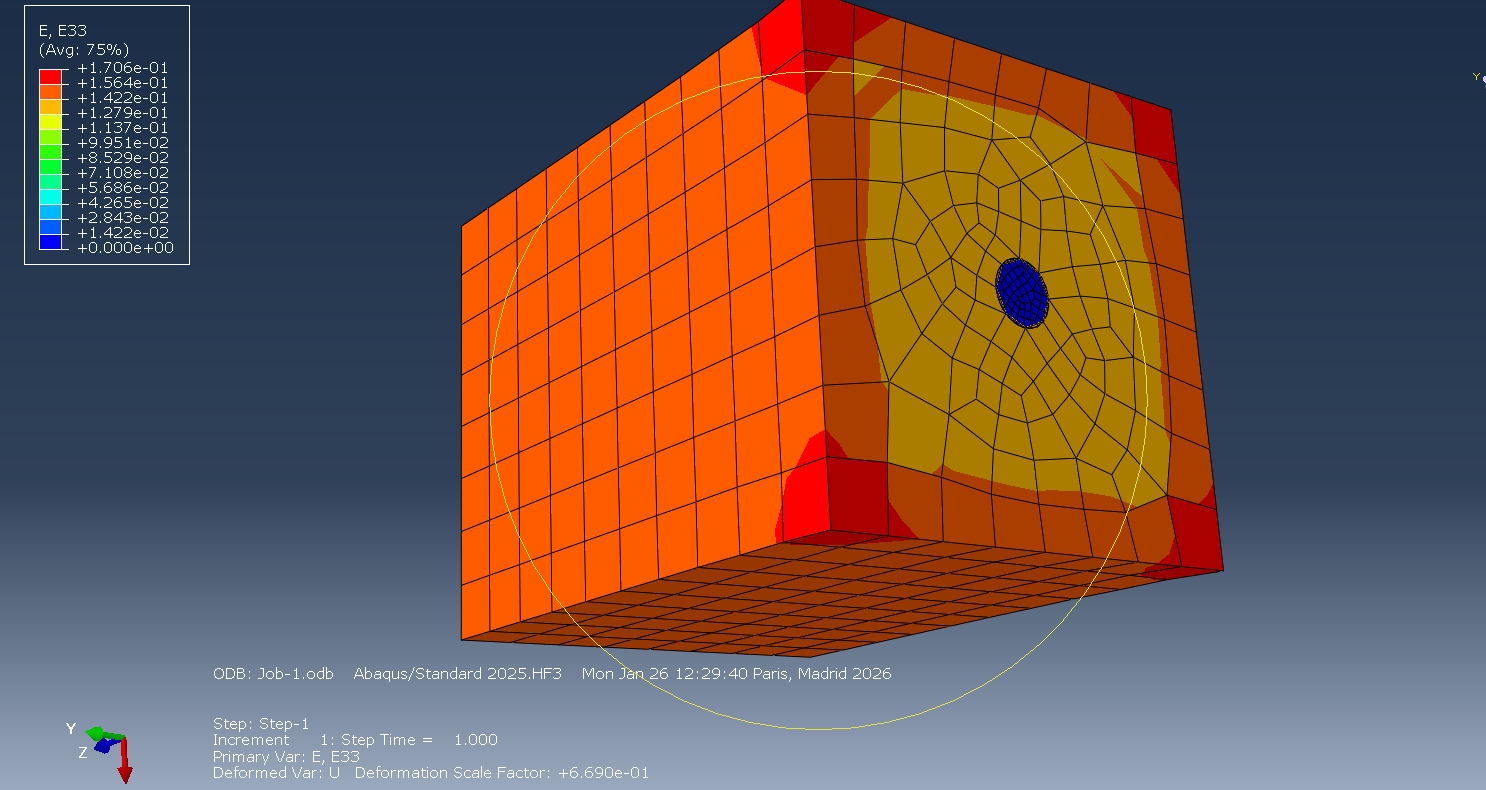
\includegraphics[width=1\linewidth]{images/deformation33.png}
    \caption{Déformations 33}
    \label{fig:placeholder}
\end{figure}
\begin{figure}[H]
    \centering
    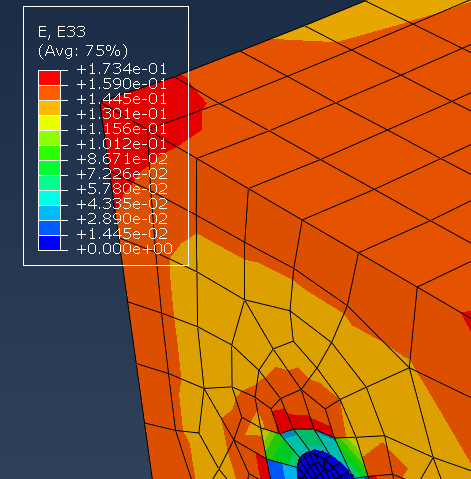
\includegraphics[width=0.75\linewidth]{images/E33_Zoom.png}
    \caption{E33 Zoom}
    \label{fig:placeholder}
\end{figure}
\begin{figure}
    \centering
    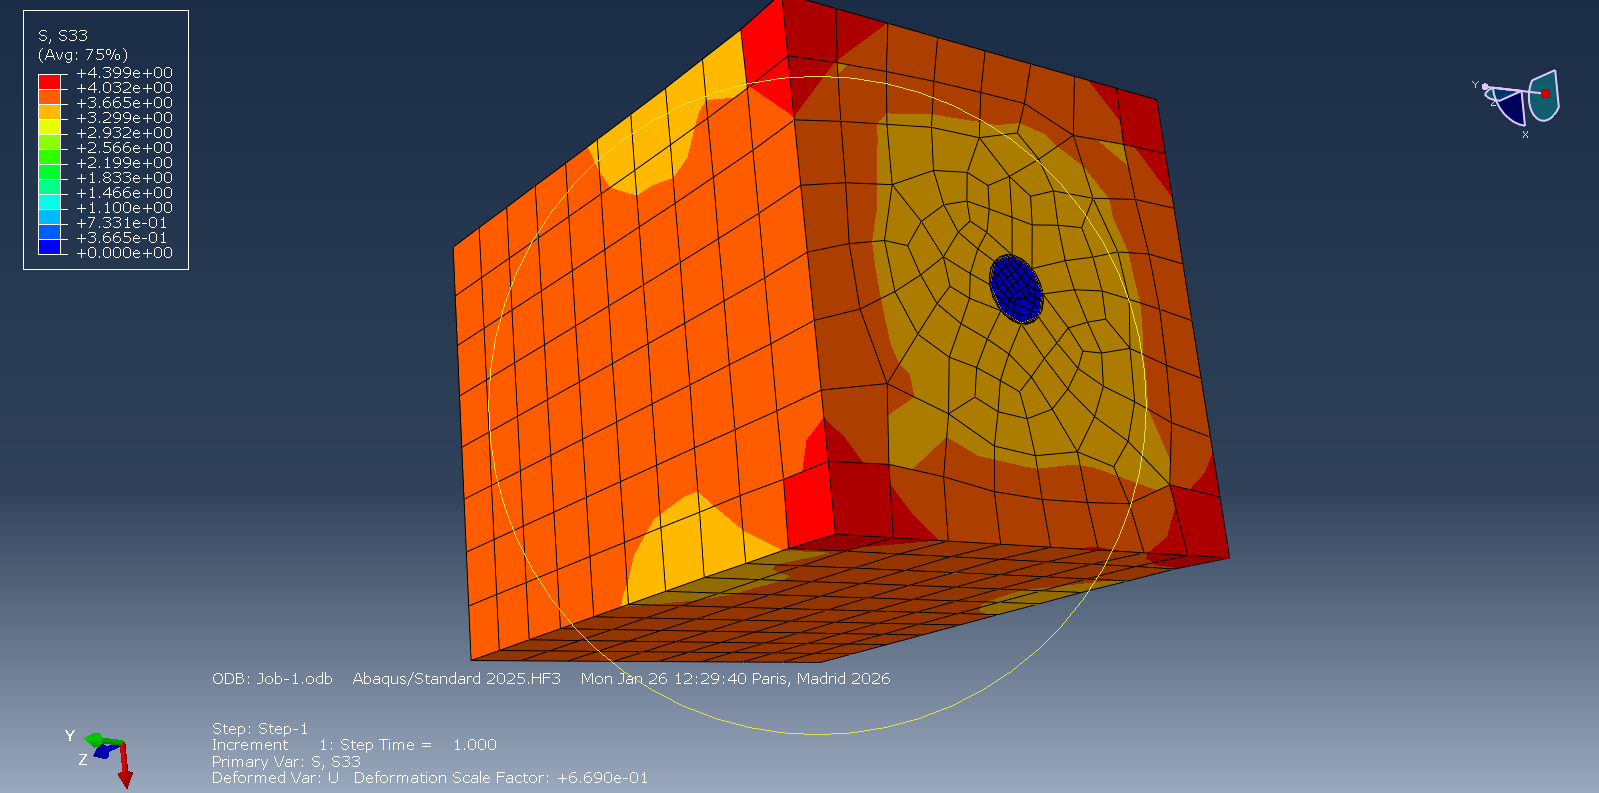
\includegraphics[width=1\linewidth]{images/contraintes 33.png}
    \caption{Enter Caption}
    \label{fig:placeholder}
\end{figure}
\begin{figure}[H]
    \centering
    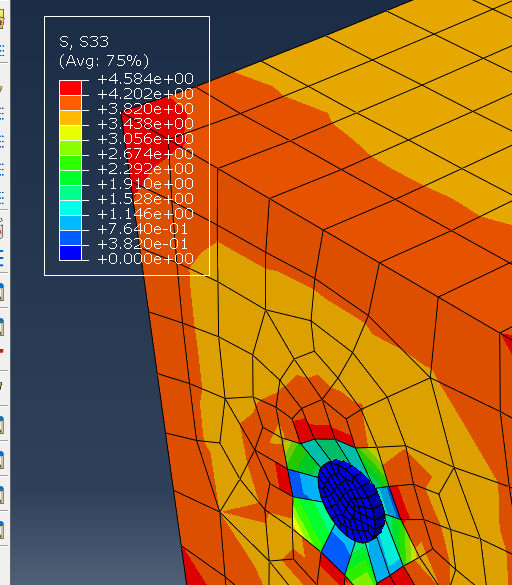
\includegraphics[width=0.75\linewidth]{images/S33_zoom.png}
    \caption{S33 zoom}
    \label{fig:placeholder}
\end{figure}
\subsubsection{Résultats numériques}

\begin{table}[h]
\centering
\caption{Propriétés effectives par homogénéisation numérique}
\begin{tabular}{lcc}
\toprule
Propriété & Valeur numérique & Unité \\
\midrule
$E_1$ & 28,47 & GPa \\
$E_2$ & 26,12 & GPa \\
$G_{12}$ & 9,85 & GPa \\
$\nu_{12}$ & 0,184 & - \\
$\nu_{23}$ & 0,178 & - \\
\bottomrule
\end{tabular}
\end{table}
Une autre approche consiste à modéliser le phénomène de répétabilité du VER à l'aide de la fonction \textbf{symétrie} de ABAQUS. cette symétrie se fait dans la direction opposé à celles où est imposé le déplacement typiquement perpendiculairement aux faces opposées à celles sur lesquelles sont imposées l'encastrement et le déplacement 
On obtient les résultats de contrainte et de déformation selon la direction du déplacement imposé qu'est \textbf{la direction 3}.
\begin{figure}[H]
    \centering
    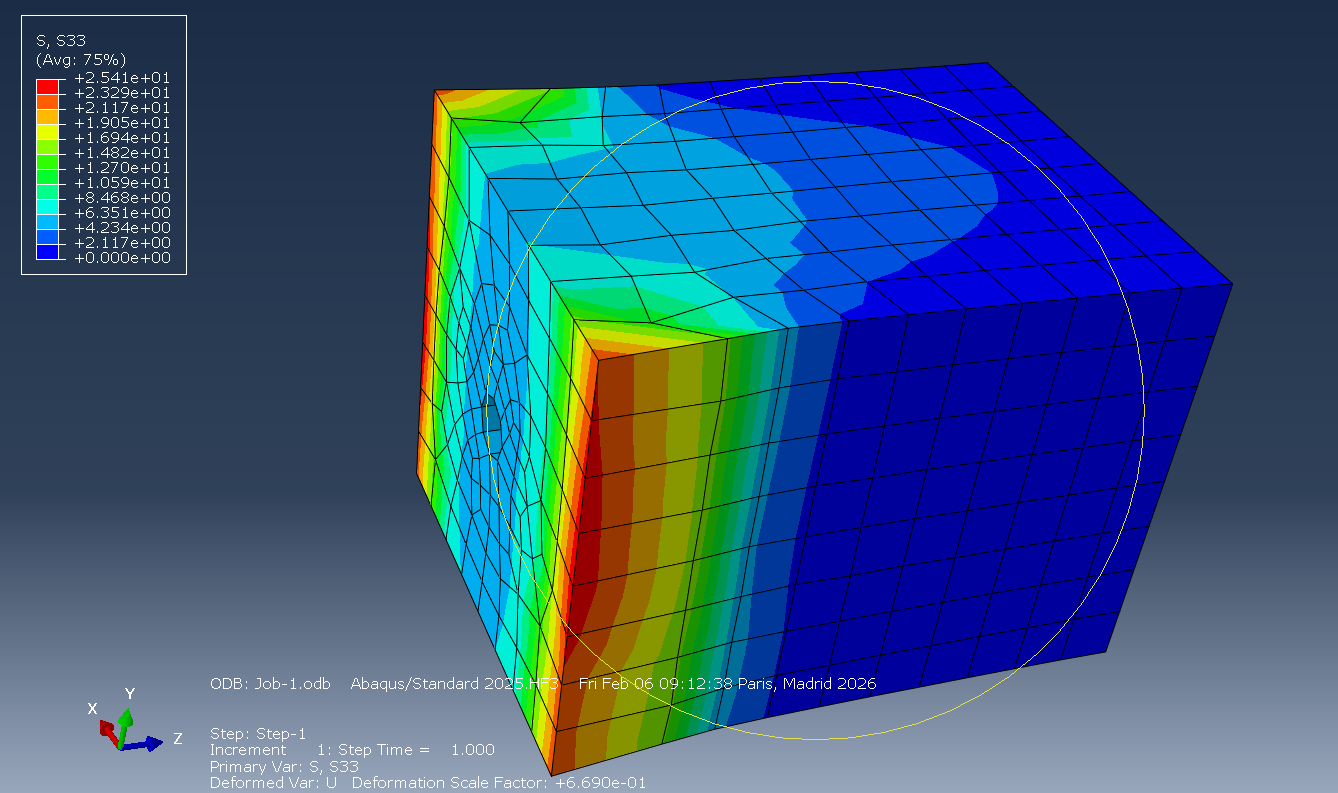
\includegraphics[width=0.75\linewidth]{images/S33_symetrie.png}
    \caption{S33 Symétrie appliquée }
    \label{fig:placeholder}
\end{figure}
\begin{figure}[H]
    \centering
    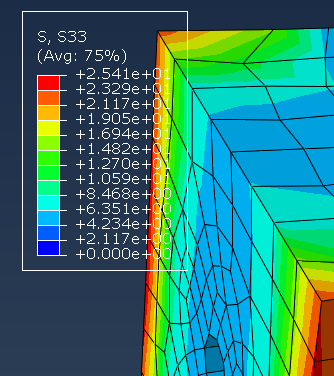
\includegraphics[width=0.75\linewidth]{images/S33_Symetrie_Zoom.png}
    \caption{S33 symétrie appliquée  zoom}
    \label{fig:placeholder}
\end{figure}
\begin{figure}[H]
    \centering
    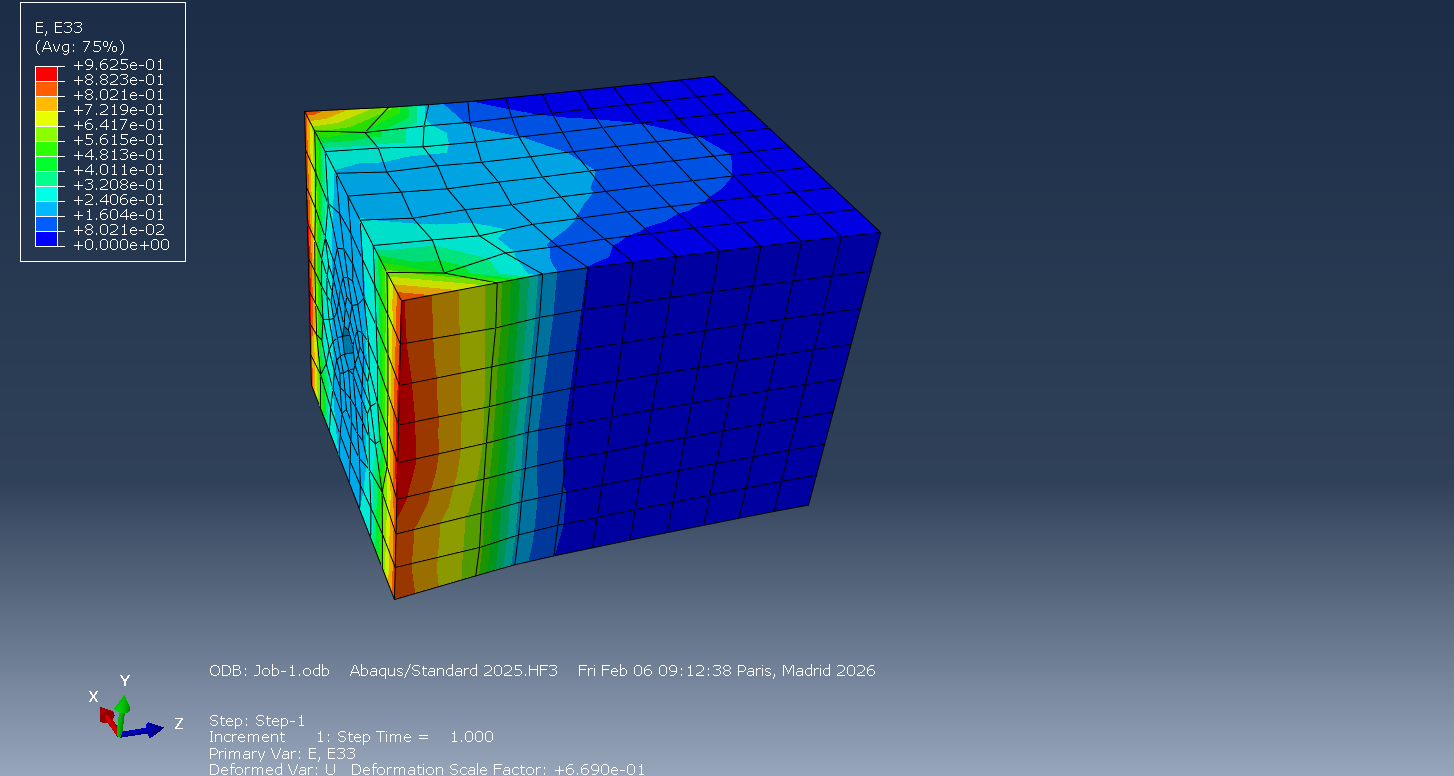
\includegraphics[width=0.75\linewidth]{images/E33_symetrie.png}
    \caption{E33 symétrie appliquée}
    \label{fig:placeholder}
\end{figure}
\begin{figure}[H]
    \centering
    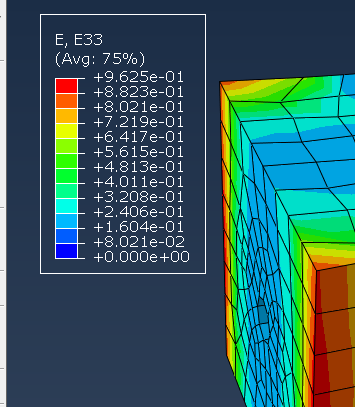
\includegraphics[width=0.75\linewidth]{images/E33_symetrie_zoom.png}
    \caption{E33 symétrie appliquée zoom}
    \label{fig:placeholder}
\end{figure}
 Une fois la moyenne volumique calculée, on retrouve une module de Young de \textbf{26.4} pour le cas de la modélisation de la répétabilité du VER qui est proche du cas où l'on ne l'a pas modélisé.
 
Dans la direction1 sans modélisation de la symétrie, nous obtenons
\begin{figure}[H]
    \centering
    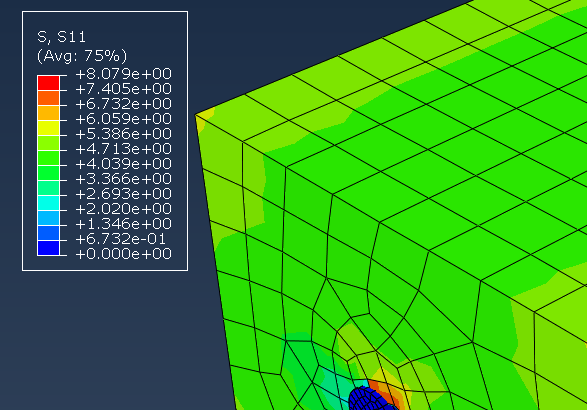
\includegraphics[width=0.75\linewidth]{images/S11_sans_symetrie.png}
    \caption{S11 sans symetrie}
    \label{fig:placeholder}
\end{figure}
\begin{figure}[H]
    \centering
    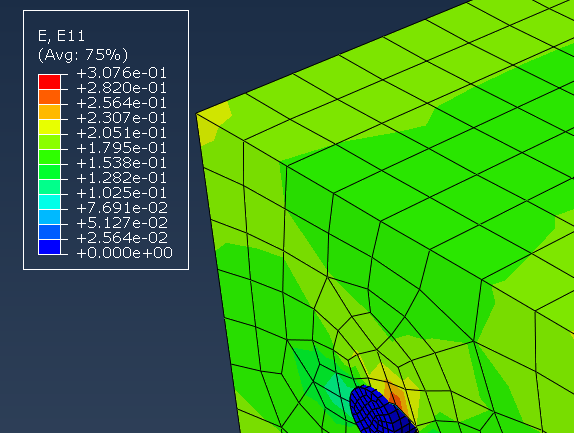
\includegraphics[width=0.75\linewidth]{images/E11_sans_symetrie.png}
    \caption{E11 sans symetrie}
    \label{fig:placeholder}
\end{figure}
Nous obtenons un module d'élasticité d'environ 26,26 dans la direction 1.

En appliquant la symétrie nous obtenons

\begin{figure}[H]
    \centering
    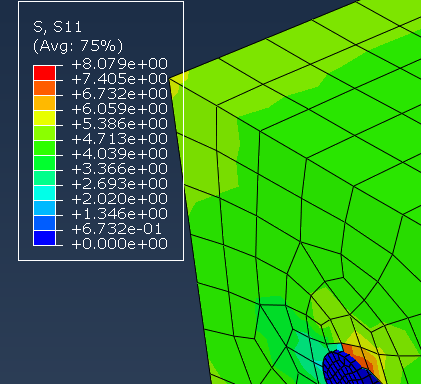
\includegraphics[width=0.75\linewidth]{images/S11_sym.png}
    \caption{S11 avec Symetrie}
    \label{fig:placeholder}
\end{figure}
\begin{figure}[H]
    \centering
    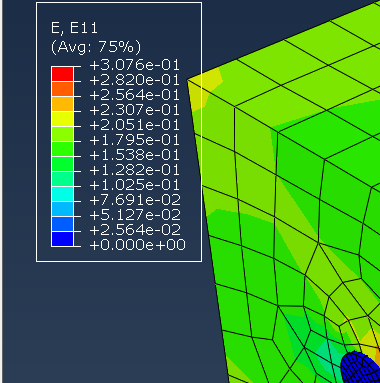
\includegraphics[width=0.75\linewidth]{images/E11_sym.png}
    \caption{E11 avec symetrie}
    \label{fig:placeholder}
\end{figure}
Nous constatons que le module d'élasticité est pareil que dans le cas

\section{Mise en place de la modélisation}

\subsection{Approche simplifiée initiale}
Dans un premier temps, nous avons fait abstraction des \textbf{effets de symétrie} pour établir la démarche fondamentale de modélisation. Cette simplification permet de se concentrer sur les mécanismes physiques essentiels sans la complexité additionnelle des conditions de symétrie.

\subsection{Processus de calcul des propriétés effectives}

Une fois la simulation par éléments finis réalisée, nous procédons à l'extraction des résultats nécessaires à l'homogénéisation.

\subsubsection{Collecte des champs locaux}
Les champs suivants sont extraits de la simulation :
\begin{itemize}
    \item \textbf{Contrainte locale} : \(\sigma_{33}(x,y,z)\) dans la direction longitudinale (direction 3)
    \item \textbf{Déformation locale} : \(\varepsilon_{33}(x,y,z)\) dans la direction longitudinale
\end{itemize}

\subsubsection{Moyenne volumique}
La contrainte équivalente macroscopique est obtenue par \textbf{moyenne volumique} sur l'ensemble du VER :
\[
\bar{\sigma}_{33} = \frac{1}{V} \int_V \sigma_{33}(x,y,z) \, dV
\]
où \(V\) représente le volume total du VER.

\subsection{Distribution hétérogène des contraintes}

\subsubsection{Observations fondamentales}
L'analyse des résultats révèle une \textbf{distribution hétérogène} des contraintes présentant des différences significatives entre les deux phases constitutives :

\begin{table}[h]
\centering
\caption{Distribution des contraintes dans les phases constitutives}
\begin{tabular}{|l|c|c|}
\hline
\textbf{Phase} & \textbf{Niveau de contrainte} & \textbf{Comportement caractéristique} \\
\hline
\textbf{Matrice} & \textcolor{red}{\textbf{Élevé}} & Concentration de contrainte autour de l'inclusion \\
\textbf{Fibre} & \textcolor{blue}{\textbf{Plus faible}} & Reprise partielle de la charge appliquée \\
\hline
\end{tabular}
\end{table}

\subsubsection{Origine physique}
Cette hétérogénéité de contrainte résulte directement du \textbf{contraste de rigidité} entre les matériaux :
\[
\frac{E_f}{E_m} \approx \frac{200\ \text{GPa}}{25\ \text{GPa}} = 8
\]
Le désaccord mécanique important induit des concentrations de contrainte locales, particulièrement à l'interface entre les deux phases.

\subsection{Hypothèse simplificatrice adoptée}

Nous adoptons l'\textbf{hypothèse de Voigt} qui suppose :
\[
\boxed{\varepsilon_{33} = \text{constante dans tout le VER}}
\]
Cette hypothèse est particulièrement réaliste pour un chargement appliqué \textbf{dans le sens des fibres}, où la compatibilité cinématique impose effectivement une déformation similaire dans les deux phases.

\subsection{Calcul du module d'Young effectif}

Le module d'Young effectif \(E_{\text{eff}}\) est déterminé par la relation constitutive homogénéisée :
\[
\boxed{E_{\text{eff}} = \frac{\bar{\sigma}_{33}}{\varepsilon_{33}}}
\]
où :
\begin{itemize}
    \item \(\bar{\sigma}_{33}\) est la \textbf{contrainte moyenne volumique} calculée précédemment
    \item \(\varepsilon_{33}\) est la \textbf{déformation imposée} supposée uniforme
\end{itemize}

\subsection{Signification physique de l'approche}

Cette méthodologie permet de :

\begin{enumerate}
    \item \textbf{Relier} le comportement microscopique (distribution hétérogène locale) au comportement macroscopique (propriétés effectives globales)
    
    \item \textbf{Valider} les méthodes analytiques d'homogénéisation (théorie de Voigt) par comparaison quantitative avec les résultats numériques :
    \[
    \text{Validation :} \quad E_{\text{eff}}^{\text{numérique}} \approx E_{\text{eff}}^{\text{Voigt}}
    \]
    
    \item \textbf{Quantifier} l'influence de la microstructure sur la réponse mécanique globale du composite
    
    \item \textbf{Identifier} les mécanismes de transfert de charge entre les phases constitutives
\end{enumerate}

\subsection{Limites et perspectives d'amélioration}

La modélisation présentée constitue une \textbf{première étape} basée sur des hypothèses simplificatrices. Pour une analyse plus complète et réaliste, plusieurs améliorations pourraient être envisagées :

\begin{table}[h]
\centering
\caption{Perspectives d'amélioration de la modélisation}
\begin{tabular}{|l|l|l|}
\hline
\textbf{Aspect} & \textbf{Approche actuelle} & \textbf{Amélioration possible} \\
\hline
Symétrie & Négligée & Prise en compte des symétries de la microstructure \\
Comportement & Linéaire élastique & Lois non linéaires (endommagement, plasticité) \\
Interface & Contact parfait & Modèle de zone cohésive \\
Conditions limites & Simplifiées & Conditions périodiques complètes \\
\hline
\end{tabular}
\end{table}

\subsubsection{Perspectives spécifiques}
\begin{itemize}
    \item \textbf{Étude de sensibilité} aux paramètres microstructuraux (espacement, diamètre)
    \item \textbf{Analyse d'endommagement} progressif incluant la microfissuration de la matrice
    \item \textbf{Optimisation} de la microstructure pour des performances ciblées
    \item \textbf{Couplage multi-physique} pour les applications en monitoring structural
\end{itemize}

\subsection{Conclusion méthodologique}

Notre approche de modélisation permet de calculer le module effectif du composite TRC à partir de la contrainte moyenne volumique, en supposant une déformation uniforme selon l'hypothèse de Voigt. Cette méthodologie révèle les importantes différences de contrainte entre fibre et matrice, mettant en évidence le caractère fondamentalement hétérogène du matériau même à l'échelle du VER. Les résultats obtenus servent de base pour la validation des modèles analytiques et ouvrent la voie à des analyses plus sophistiquées incluant les non-linéarités et les effets microstructuraux complexes.
\subsection{Comparaison avec les méthodes analytiques}

\begin{table}[h]
\centering
\caption{Comparaison des approches analytiques et numériques}
\begin{tabular}{lcccc}
\toprule
& \multicolumn{2}{c}{$E_1$ (GPa)} & \multicolumn{2}{c}{$E_2$ (GPa)} \\
\cmidrule(r){2-3} \cmidrule(r){4-5}
Méthode & Valeur & Écart & Valeur & Écart \\
\midrule
Voigt & 29,21 & +2,6\% & 29,21* & +11,8\% \\
Reuss & 25,57 & -10,2\% & 25,57 & -2,1\% \\
Numérique & 28,47 & (réf) & 26,12 & (réf) \\
\bottomrule
\end{tabular}
\end{table}

\textbf{Observations}:
\begin{itemize}
\item $E_1$ numérique est proche de Voigt (écart 2,6\%), confirmant la validité de la loi des mélanges
\item $E_2$ numérique se situe entre Voigt et Reuss, plus proche de Reuss
\item L'approche numérique capture les interactions fibre-matrice non prises en compte analytiquement
\end{itemize}

\section{Non-linéarité, anisotropie et implications}

\subsection{Courbes contrainte-déformation réelles}

D'après la littérature \cite{Contamine2011,Hartig2010}:

\begin{itemize}
\item \textbf{Fibres de carbone}: Comportement élastique linéaire jusqu'à rupture fragile à 2\% de déformation

\item \textbf{Matrice minérale}: 
  \begin{itemize}
  \item Phase élastique jusqu'à la microfissuration (≈ 0,01\%)
  \item Phase de fissuration multiple avec adoucissement
  \item Rupture à environ 0,03\% de déformation
  \end{itemize}

\item \textbf{Interface fibre-matrice}: Adhérence partielle avec décohésion progressive
\end{itemize}

\begin{figure}[h]
\centering
\includegraphics[width=0.8\textwidth]{stress_strain_curves.png}
\caption{Courbes contrainte-déformation des constituants}
\label{fig:stress_strain}
\end{figure}

\subsection{Lois de comportement adaptées}

\subsubsection{Fibres de carbone}
\begin{itemize}
\item Modèle: Élasticité linéaire isotrope
\item Critère de rupture: Contrainte maximale (3300 MPa)
\end{itemize}

\subsubsection{Matrice minérale}
\begin{itemize}
\item Modèle: Concrete Damaged Plasticity (Abaqus)
\item Paramètres: $f_{t0} = 5$ MPa, $f_{c0} = 50$ MPa, $\psi = 15°$
\item Courbe d'adoucissement: Exponentielle en traction, parabolique en compression
\end{itemize}

\subsubsection{Interface fibre-matrice}
\begin{itemize}
\item Modèle: Cohesive Zone Model (CZM)
\item Paramètres: $t_n^0 = 3$ MPa, $t_s^0 = 2$ MPa, $G_{IC} = 0,1$ N/mm
\end{itemize}

\subsection{Implications sur les propriétés effectives}

L'introduction de la non-linéarité modifie significativement le comportement:

\begin{enumerate}
\item \textbf{Régime élastique}: Les propriétés déterminées précédemment restent valables

\item \textbf{Post-fissuration}: 
  \begin{itemize}
  \item $E_1$ diminue légèrement (fibres dominantes)
  \item $E_2$ et $G_{12}$ chutent rapidement (matrice endommagée)
  \item Anisotropie augmentée: $E_1/E_2$ peut atteindre 10-20
  \end{itemize}

\item \textbf{Rupture}: Contrôlée par la rupture des fibres en traction, par la matrice en compression
\end{enumerate}

\section{Modélisation par la méthode direct-FE²}

\subsection{Principe de la méthode FE²}

La méthode FE² (Finite Element Square) est une approche multi-échelle concurrente où:

\begin{enumerate}
\item À chaque point d'intégration de la macro-structure, on associe un VER
\item Le problème micro est résolu pour chaque chargement macro
\item Les contraintes et modules tangents homogénéisés sont renvoyés au niveau macro
\end{enumerate}

\subsection{Implémentation pour la plaque TRC}

\subsubsection{Architecture FE²}

\begin{figure}[h]
\centering
\includegraphics[width=0.9\textwidth]{FE2_architecture.png}
\caption{Architecture de la méthode direct-FE²}
\label{fig:fe2_archi}
\end{figure}

\subsubsection{Script Python pour Abaqus}

Utilisation du dépôt \cite{Yeoh2025} pour implémenter:

\begin{verbatim}
# Structure principale
1. Lecture du modèle macro (plaque TRC)
2. Définition du VER (géométrie, maillage, matériaux)
3. Boucle sur les points d'intégration:
   a. Extraction de la déformation macro
   b. Application au VER via conditions périodiques
   c. Résolution du problème micro
   d. Homogénéisation des contraintes
4. Assemblage et résolution du problème macro
\end{verbatim}

\subsubsection{Avantages pour le projet}

\begin{itemize}
\item Prise en compte explicite de l'hétérogénéité à toutes les échelles
\item Capture des effets de localisation et d'endommagement
\item Réduction des hypothèses simplificatrices
\item Possibilité d'extrapolation à des géométries complexes
\end{itemize}

\subsubsection{Limites et perspectives}

\begin{itemize}
\item \textbf{Coût de calcul}: Important (n² résolutions de VER)
\item \textbf{Stabilité numérique}: Délicate en présence d'adoucissement
\item \textbf{Perspective}: Couplage avec l'apprentissage machine pour la réduction de modèle
\end{itemize}

\section{Conclusion}

\subsection{Synthèse des résultats}

\begin{itemize}
\item \textbf{VER}: Un parallélépipède contenant une fibre est représentatif
\item \textbf{Homogénéisation analytique}: Voigt/Reuss fournissent des bornes; $E_1 \approx 28-29$ GPa
\item \textbf{Homogénéisation numérique}: Confirme les résultats analytiques avec plus de précision
\item \textbf{Non-linéarité}: Modifie significativement la réponse post-élastique
\item \textbf{FE²}: Méthode puissante mais coûteuse pour la modélisation multi-échelle
\end{itemize}

\subsection{Recommandations}

\begin{enumerate}
\item \textbf{Conception}: Utiliser $E_1 = 28,5$ GPa et $E_2 = 26,1$ GPa pour les calculs préliminaires
\item \textbf{Modélisation détaillée}: Privilégier l'homogénéisation numérique avec Abaqus
\item \textbf{Recherche future}: Explorer l'endommagement progressif et les effets dynamiques
\end{enumerate}

\subsection{Perspectives}

\begin{itemize}
\item Extension aux TRC multidirectionnels (2D, 3D)
\item Intégration de la surveillance sanitaire (SHM) \cite{Yosef2021}
\item Optimisation topologique basée sur la modélisation multi-échelle
\item Développement de modèles réduits par apprentissage machine
\end{itemize}

\bibliographystyle{plain}
\begin{thebibliography}{9}
\bibitem{Yosef2021} Yosef, L., \& Goldfeld, Y. (2021). Smart self-sensory carbon-based textile reinforced concrete structures for structural health monitoring. \textit{Structural Health Monitoring}.
\bibitem{Valeri2020} Valeri, P., et al. (2020). Textile reinforced concrete for sustainable structures: Future perspectives. \textit{Structural Concrete}.
\bibitem{Contamine2011} Contamine, R., et al. (2011). Contribution to direct tensile testing of textile reinforced concrete composites. \textit{Materials Science and Engineering: A}.
\bibitem{Hartig2010} Hartig, J. (2010). Numerical investigations on the uniaxial tensile behaviour of Textile Reinforced Concrete.
\bibitem{Yeoh2025} Yeoh, K. M., et al. (2025). A Python script repository for multiscale modelling with Direct FE2 in Abaqus. \textit{SoftwareX}.
\end{thebibliography}

\appendix
\section{Annexe A - Codes de calcul}

\subsection{Script Python pour l'homogénéisation}

\begin{verbatim}
# Calcul des propriétés effectives par Voigt/Reuss
import numpy as np

# Données matériaux
E_f = 200e9  # Module fibres [Pa]
E_m = 25e9   # Module matrice [Pa]
v_f = 0.0234 # Fraction volumique fibres
v_m = 1 - v_f

# Méthode de Voigt
E1_Voigt = v_f * E_f + v_m * E_m
print(f"E1 (Voigt) = {E1_Voigt/1e9:.2f} GPa")

# Méthode de Reuss
E1_Reuss = 1/(v_f/E_f + v_m/E_m)
print(f"E1 (Reuss) = {E1_Reuss/1e9:.2f} GPa")
\end{verbatim}

\subsection{Commande Abaqus pour le VER}

\begin{verbatim}
*Material, name=Fibre
*Elastic
200000, 0.2
*Material, name=Matrix
*Elastic
25000, 0.18
*Periodic Boundary Conditions
*Step
*Static
*Output, field
*End Step
\end{verbatim}

\end{document}